% =====================================================================
% EXEMPLOS DE USO DOS COMANDOS  (nao faz parte da entrega)
% Copie o trecho que precisar para a sua secao.
% =====================================================================
\newpage
\section*{Exemplos de uso (apagar antes de entregar)}

\subsection*{1. Desenhar um estado}
\begin{figure}[H]
\centering
\begin{tikzpicture}
  % \bl{ponto p}{nivel l}{comprimento}{nome}
  \mesa
  \bl{0}{0}{2}{c}\bl{3}{0}{1}{a}\bl{5}{0}{1}{b}\bl{3}{1}{3}{d}
  \rot{$S_0$}
\end{tikzpicture}
\caption{Um estado.}
\end{figure}

\subsection*{2. Dois estados com uma ação entre eles}
\begin{figure}[H]
\centering
\begin{tikzpicture}
  \begin{scope}\mesa
    \bl{0}{0}{2}{c}\bl{3}{0}{1}{a}\bl{5}{0}{1}{b}\bl{3}{1}{3}{d}\rot{$S_0$}
  \end{scope}
  \draw[-{Stealth}] (3.3,0.5) -- node[above,font=\scriptsize]{move(d,c,0)} (5.1,0.5);
  \begin{scope}[xshift=5.4cm]\mesa
    \bl{0}{0}{2}{c}\bl{3}{0}{1}{a}\bl{5}{0}{1}{b}\bl{0}{1}{3}{d}\rot{$S_1$}
  \end{scope}
\end{tikzpicture}
\caption{Uma transição.}
\end{figure}

\subsection*{3. Tabela de passos (ação, pré-condições, ADD, DEL)}
\begin{table}[H]
\centering\small
\renewcommand{\arraystretch}{1.25}
\begin{tabularx}{\textwidth}{@{}p{2.3cm} X X X@{}}
\toprule
Ação & Pré-condições (verificadas) & ADD & DEL\\
\midrule
$A_1$: move(d,c,0)\newline $t=0$ &
$\clr(d)$; \dots &
$\at(d,0)$, $\on(d,c)$, \dots &
$\at(d,3)$, $\on(d,a)$, \dots\\
\bottomrule
\end{tabularx}
\caption{Execução manual passo a passo.}
\end{table}

\subsection*{4. Fórmulas}
\begin{align}
&\clr(b,t) \leftrightarrow \forall s,l\,\bigl(\cov(b,s,l,t)\rightarrow
  \esp(b,s,t)\bigr) \tag{A5b}
\end{align}
Vínculo causal no texto: $A_1\xrightarrow{\;\clr(a)\;}A_2$. Ordem: $A_1\prec A_2$.

\subsection*{5. Grafo de ordem parcial}
\begin{figure}[H]
\centering
\begin{tikzpicture}[node distance=1.0cm,
  acao/.style={draw,rounded corners,fill=cora!12,minimum width=4.4cm,
               minimum height=0.75cm,font=\small},
  lig/.style={-{Stealth},thick}]
  \node[acao,fill=black!6] (ini) {Início};
  \node[acao,below=of ini] (a1) {$A_1$: move(d,c,0)};
  \node[acao,below=of a1,fill=black!6] (fim) {Fim};
  \draw[lig] (ini) -- node[right,font=\footnotesize]{\ $\clr(d)$} (a1);
  \draw[lig] (a1) -- node[right,font=\footnotesize]{\ \dots} (fim);
\end{tikzpicture}
\caption{Grafo de ordem parcial.}
\end{figure}

\subsection*{6. Comandos e saída de terminal}
\begin{lstlisting}
$ python3 ../bw2cnf_var.py --cenario 1
Gerado: ... variaveis, ... clausulas (T=4)
\end{lstlisting}

\subsection*{7. Tabela simples}
\begin{center}\small
\begin{tabular}{@{}lll@{}}
\toprule
Coluna 1 & Coluna 2 & Coluna 3\\
\midrule
a & b & c\\
\bottomrule
\end{tabular}
\end{center}
